\documentclass{article}
\usepackage{polski}
\usepackage[utf8]{inputenc}
\usepackage{graphicx}
\usepackage{amsmath}
\usepackage{amssymb}
\usepackage{mathtools}
\usepackage{hyperref}

\title{Teoria Regulacji - Ćwiczenia}
\author{Jan Bronicki 249011 \\
        Denis Firat 249031  \\
        Borys Staszczak 248958 }
\date{}

\begin{document}

\maketitle
\begin{center}
    Zadanie 4, Lista 3
\end{center}

\section{Opracowanie teoretyczne kryterium Nyquista}
\subsection{Wstęp}
Opracowane przez amerykańskiego inżyniera Harry'ego Nyquista na potrzeby wzmacniaczy z sprzężeniem zwrotnym kryterium, nazywane dziś "Kryterium Nyquista" jest narzędziem niezwykle przydatnym, ponieważ pozwala nam określać stabilność systemów  z sprzężeniem zwrotnym na podstawie charakterystyki amplitudowo-fazowej transmitancji systemu otwartego! Osiągnięcie to jest dużo bardziej ekscytujące, gdy jest się świadomym, że wystarczy dodać 1 do mianownika transmitancji i zmienia to już bieguny i zera transmitancji. Natomiast charakterystyka amplitudowo fazowa po prostu przesuwa się o jeden w prawo! Prawda, że bardziej ekscytujące? Jeszcze ciekawsze są dowody na twierdzenia Nyquista. Dogłębne zrozumienie kryterium Nyquista, zajęło nam 3 dni i szło jak krew z nosa, więc dołożę wszelkich starań by udowodnić, że NAPRAWDĘ to rozumiemy. Dodać muszę, że większość wiedzy zawartej w tym opracowaniu teoretycznym pochodzi z książki "Teoretyczne podstawy automatyki" prof. Greblickiego. Książka dostępna pod tym adresem za darmo \url{http://diuna.ict.pwr.wroc.pl/greblicki/BOOKS/PDF/2001-Teoretyczne\%20podstawy\%20automatyki.pdf} Książka Profesora okazała się zbawieniem, ponieważ zapis matematyczny i tłumaczenie Profesora, jest niezwykle czytelne i zrozumiałe. W zrozumieniu kryterium Nyquista pomógł nam również kanał Brian Douglas na yt, oraz za duże ilości filmików hindusów.\newpage
\subsection{Przedstawienie systemów z sprzężeniem zwrotnym}
Schemat systemu z sprzężeniem zwrotnym, później nazywanym \\CLS(closed loop system):\\
\begin{figure}
    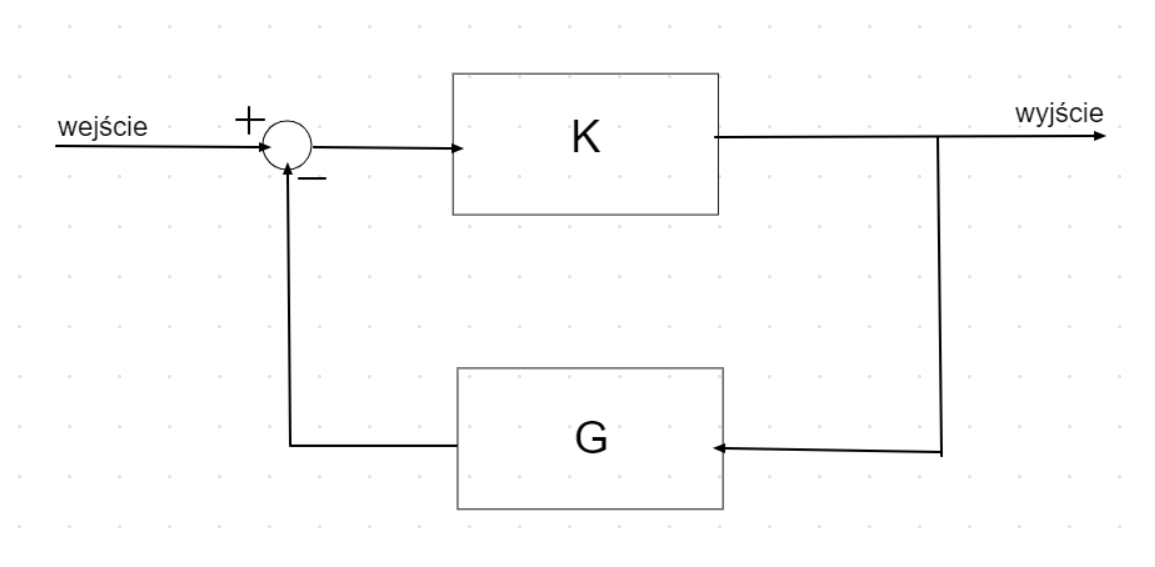
\includegraphics[width=12cm]{cls.png}
    \centering
\end{figure}
\\
Transmitancja takiego systemu ma postać
$$K_z(s)=\frac{K(s)}{1+K(s)G(s)}$$
Schemat systemu z otwartym sprzężeniem zwrotnym, później nazywanym OLS(open loop system)
\begin{center}
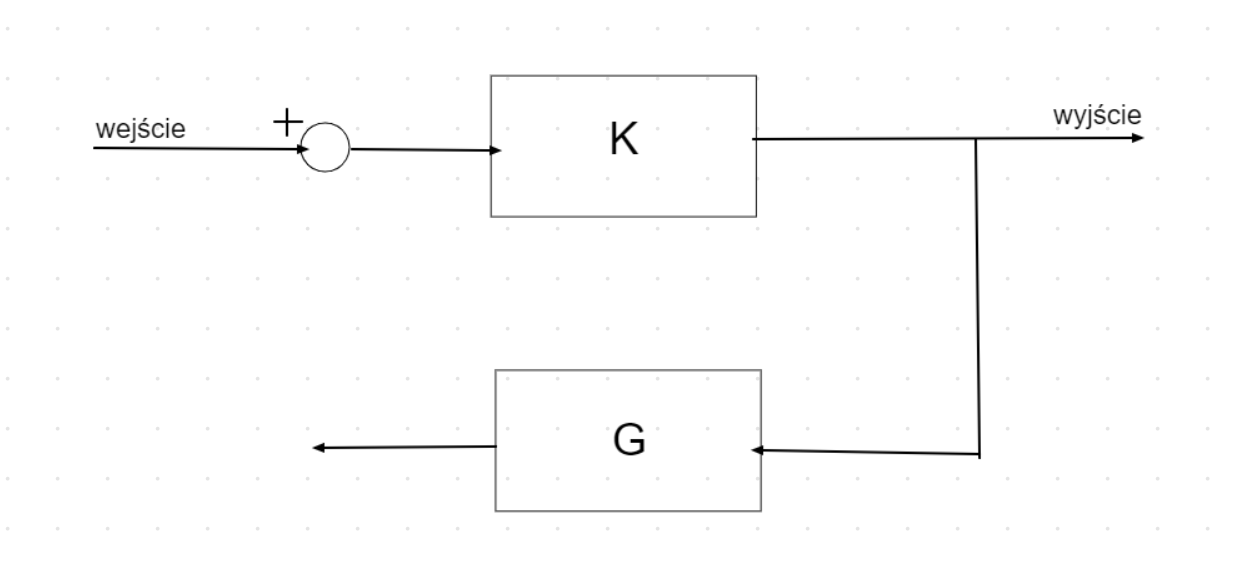
\includegraphics[width=12cm]{ols.png}    
\end{center}
Transmitancja takiego systemu ma postać
$$K_O(s)=K(s)G(s)$$
\newpage
\subsection{Pochodzenie kryterium Nyquista}
Warto teraz dodać, że kryterium Nyquista ma charakter częstotliwości ponieważ, badamy stabilność dla $s=j\omega$, gdzie zmienna jest pulsacja omega. Kryterium Nyquista bazuje na kryterium Michajłowa, a dokładniej na tym jak bieguny i ich położenie wpływa na $\Delta arg(M(j\omega))$. Stabilność CLS zależy od jego mianownika czyli 1+K(s)G(s), czyli zależy od OLS "przesuniętego" o jeden. Kryterium Nyquista, wymaga od nas określenia najpierw stabilności OLS, a następnie z pomocą odpowiedniego twierdzenia kryterium orzekamy stabilność CLS.\\
\subsection{Wspomnienie Michajłowa}
\begin{center}
Jak to się dzieje, że bieguny wpływają na $\Delta arg(M(j\omega))$ ?\\Najpierw zapiszmy mianownik transmitancji w takiej postaci:
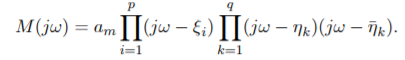
\includegraphics[]{mich1.png}\\
W takim razie argument mianownika wygląda tak:
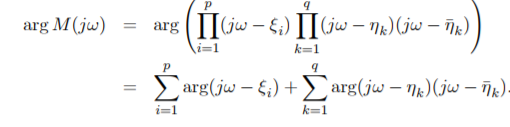
\includegraphics[]{mich2.png}
Korzystając z wzoru Eulera zauważamy, że argument mianownika to tak naprawdę suma argumentów $(j\omega -\epsilon) i (j\omega -\eta)$ gdzie $\epsilon$ to bieguny rzeczywiste, a $\eta$ to pary pierwiastków nierzeczywistych\newpage
Na poniższych ilustracjach widać graficzne przedstawienie tego ile wynosi zmiana kąta dla pierwiastków rzeczywistych i nierzeczywistych:
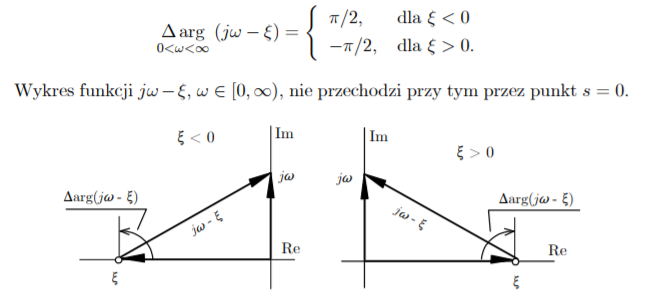
\includegraphics[]{mich3.png}
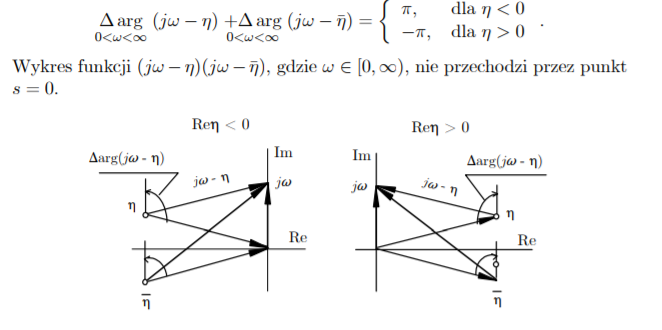
\includegraphics[]{mich4.png}
\end{center}
% \\
W skrócie bieguny rzeczywiste na lewej płaszczyźnie dodają 90 stopni, na prawej odejmują 90 stopni. Pary biegunów nierzeczywistych na lewej półpłaszczyźnie  dodają 180 stopni, a na prawej odejmują 180 stopni. Z tego wynika kryterium Michajłowa, które mówi:
\begin{center}
    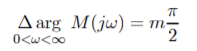
\includegraphics[]{mich5.png}
\end{center}
% \\
To tak tylko dla przypomnienia i lepszego zrozumienia Nyquista.\\
Powyższe ilustracje pochodzą z wyżej wymienionej książki porf. Greblickiego.
\subsection{Nyquist gdy mamy K(s) i G(s)}
Niestety ale Profesor w swoim opracowaniu Nyquista przedstawia go na podstawie systemu gdzie G(s)=1. Pożegnamy się na chwilę z Profesorem i na podstawie jego metodologii wyprowadzę wzory dla systemu gdzie mamy różne K i G.\\
Transmitancja CLS:(pominę (s) dla przejrzystości)\\
$$\frac{K}{1+KG}=\frac{\frac{L_K}{M_K}}{1+\frac{L_K}{M_K} \frac{L_G}{M_G}}=\frac{L_k}{M_k+\frac{L_K L_G}{M_G}}=\frac{L_K}{\frac{M_K M_G+L_K L_G}{M_G}}=$$
$$=\frac{L_K M_G}{L_K L_G + M_K M_G}$$
Transmitancja OLS:\\
$$KG=\frac{L_K L_G}{M_K M_G}=\frac{L_O}{M_O}$$
Widzimy, że wielomian charakterystyczny CLS to tak naprawdę:
$$M_Z=L_O+M_O$$
\textbf{OLS jest stabilny, sprawdzamy stabilność CLS:}\\
Kryterium Nyquista mówi nam, że gdy OLS jest stabilny, to CLS jest stabilny gdy zachowana jest własność:
$$\Delta arg(1+K_O)=0$$
Ponieważ:
$$1+K_O=\frac{L_O+M_O}{M_O}$$
$$\Delta arg(1+K_O)=\Delta arg(L_O+M_O)-\Delta arg(M_O)$$
Wiemy, że $K_O$ jest stabilne więc $\Delta arg(M_O)=m\cdot\frac{\pi}{2}$, zakładamy, że CLS jest stabilny,więc $$\Delta arg(M_O+L_O)=\Delta arg(M_Z)=m\cdot\frac{\pi}{2}$$
$$\Delta arg(1+K_O)=m\cdot\frac{\pi}{2}-m\cdot\frac{\pi}{2}=0$$
Co kończy dowód. Bardzo podobnie dochodzi się do kolejnych dwóch twierdzeń, więc na potrzeby przejrzystości, nie będę ich tutaj wyprowadzał.\\
\textbf{OLS z elementami całkującymi}
CLS jest stabilny gdy:
$$\Delta arg(1+K_O)=m_0\cdot\frac{\pi}{2}$$
Gdzie $m_0$ to ilość pierwiastków "całkujących"\\
\textbf{OLS niestabilny}\\
CLS jest stabilny gdy:
$$\Delta arg(1+K_O)=m_p\cdot\frac{\pi}{2}$$
gdzie $m_p$ to ilość pierwiastków w prawej półpłaszczyźnie liczb zespolonych\newpage

\section{Opracowanie praktyczne}

\quad Charakterystyczną cechą systemów zamkniętych jest obecność sprzężenia zwrotnego. 
Jego zadaniem jest regulowanie działania systemu przy pomocy sygnałów wyjściowych. 
Wyróżniane są dwa typy systemów zamkniętych -- ze sprzężeniem zwrotnym dodatnim oraz sprzężeniem zwrotnym ujemnym.

\begin{figure}[h!]
\centering
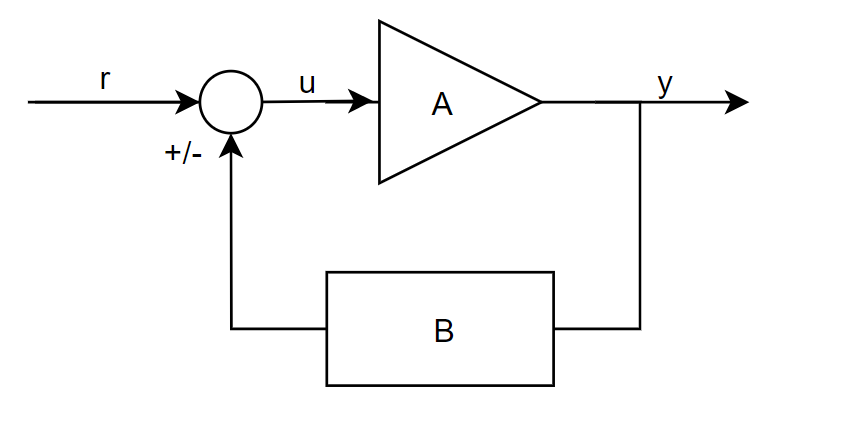
\includegraphics[scale=0.4]{feedback.png}
\caption{Model systemu zamkniętego}
\label{fig:model}
\end{figure}

\subsection{Ze sprzężeniem zwrotnym dodatnim}


\quad Układy takie zwielokrotniają wzmocnienienie sygnału co sprawia, że charakteryzują się niską stabilnością. 
W elektronice takie systemu stosuje się głównie w oscylatorach, których dzieki silnemu sprzężeniu, następuje generacja drgań.
Sprzężenie zwrotne dodatnie wykorzystuje się również w przerzutniku Schmitta, który jest włączany w obwód przekształcający analogowy sygnał wejściowy do cyfrowego sygnału wejściowego.

Codziennym przykładem sprzężenia zwrotnego dodatniego jest sytuacja w której zbliżono do głośnika mikrofon, z którego sygnał jest odtwarzany przez głośnik. Utworzona pętla znacząco wzmacnia sygnał doprowadzając do gwałtownego wzrostu głośności sprawiając, że wydobywający się z głośnika dźwięk staje staje się charakterystycznym piskiem.

\subsection{Ze sprzężeniem zwortnym ujemnym}

\quad Układy tego typu są bardzo często spotykane, charakteryzują się wysoką stabilnością ponieważ umożliwiają łatwe utrzymanie sygnału wyjściowego blisko oczekiwanych wartości. Takie systemy spotyka się nie tylko w elektronice, lecz także w naturze.\\ Prostym przykładem takiego systemu może być populacja drapiezników i ofiar. Gdy liczba drapieżników jest wysoka, maleje liczba osobników zwierząt, na które polują, w wyniku czego drapieżniki zaczynają głodować, a ich populacja się zmniejsza. System sam się reguluje poprzez zmiany w populacjach utrzymując oscylację między stałym poziomem. 

W podobny sposób organizm człowieka reguluje poziom cukru we krwi. 
Gdy poziom ten wzrasta, uwalniana jest insulina obniżająca go, natomiast gdy spadnie zbyt nisko, uwalniana jest glukoza.

W elektronice termostat jest jednym z urządzeń, w których do regulacji temperatury w pomieszczeniu wykorzystywane jest właśnie sprzężenie zwrotne. 
Urządzenie reguluje temperaturę w pomieszczeniu poprzez mierzenie jej i regulowanie ogrzewania w taki sposób by uzyskać oczekiwaną temperaturę w tym samym pomieszczeniu.

Ujemne sprzężenie zwrotne jest możliwe do zaobserwowania w spłuczce muszli klozetowej. Wewnątrz zbiornika 
znajduje się pływak połączony z zaworem, który unosi się na powierzchni wody. Po opróżnieniu pojemnika pływak
opada, wraz z poziomem wody, otwierając zawór doprowadzający wodę, zaczynając napełnianie się zbiornika.
Gdy woda osiągnie maksymalny poziom pływak zamyka zawór blokując dalszy dostęp wody. W tym systemie woda dopływająca
do zbiornika jest sygnałem wejściowym, sygnałem wyjściowym jest poziom wody, a sprzężenie zwrotne jest realizowane
przez pływak unoszący się na powierzchni wody.

\begin{figure}
    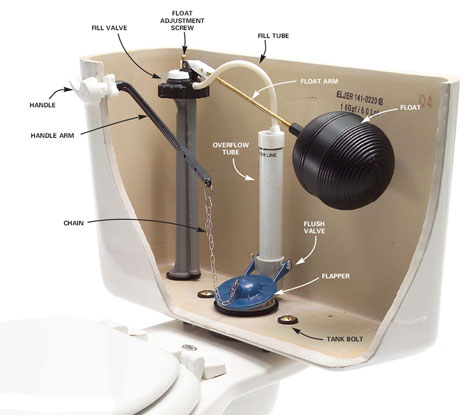
\includegraphics[width=12cm]{spluczka.jpg}
    \centering
\end{figure}
W procesorach można się spotkać ze zjawiskiem throttlingu, który ma na celu ograniczenie temperatury rdzenia przez ograniczenie częstotliwości taktowania. 
Układ stara się utrzymać bezpieczną temperaturę pracy jednoczenie zachowując jak najwyższą wydajność. 
Częstotliwość zegara jest regulowana tak by układ nie przekraczał maksymalnej bezpiecznej temperatury.
\begin{figure}
    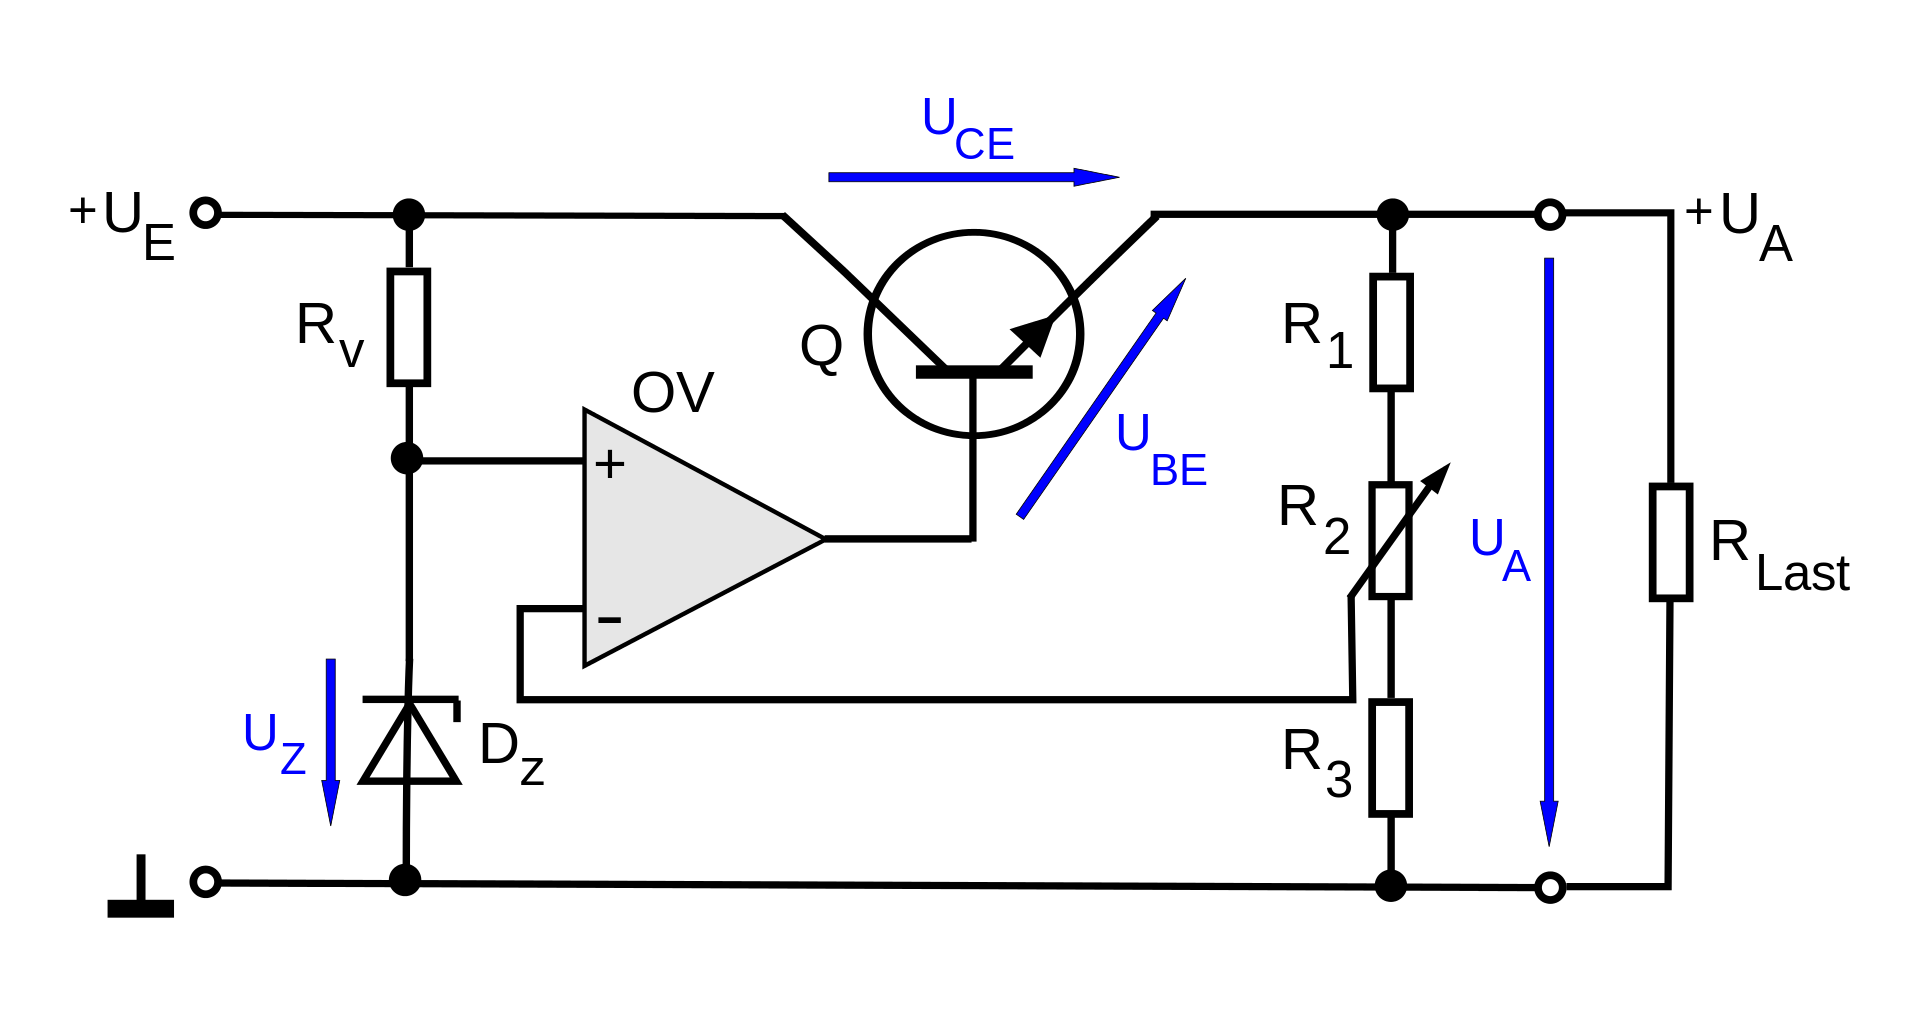
\includegraphics[width=12cm]{stab.png}
    \centering
\end{figure}

Stabilizatory napięcia zawierają w sobie układ sprzężeniem zwrotnym do utrzymywania stałego napięcia na wyjściu. Głównym elementem "Wykonawczym"
jest w tym przypadku tranzystor, a sygnał sterujący jest podawany na bazę tranzystora. Sygnał sterujący pochodzi z wzmacniacza operacyjnego, który jest
naszym "węzłem sumacyjnym". Na ujemne wejście wzmacniacza dochodzi prąd wyjściowy ograniczony potencjometrem. Od nastawy tego potencjometru zależy wartość
, na której ustabilizuje się napięcie wyjściowe.

\section{Rozwiązanie zadań}

Napisaliśmy program w Pythonie korzystający z bibliotek takich jak: SymPy, pandas, numpy, 
os oraz napisaną przez nas funkcji $Hurwitz_sp()$. Na początku tworzymy modele danych 
transmitacji za pomocą biblioteki SymPy, która słuzy do obliczeń symbolicznych w 
Pythonie, z tych modeli będziemy potem cały czas korzystać. Potem za pomocą command 
line'a w pythonie uruchamiamy Matlaba i karzemy mu wykonac pare napisanych przez nas 
funkcji, które mają na celu narysowanie Nyquista, a nastepnie zapisanie wykresów do 
plików odpowiadających kolejnym przykładom.
Dzięki bibliotece SymPy nie tylko możemy operować na symbolach matematycznych, ale możemy z nich wyciagać informacje, które będą przydatne w numerycznych komputacjach. Takie jak np. współczynniki transmitacji, którą badamy możemy zamienić na listy liczb, które następnie dzieki modułowi $os$ przekazujemy poprzez commandline do Matlaba, który z nich konstruuje u siebie taką samą transmitację, a następnie konstruuje wykres Nyquista. Dzięki SymPy'owi jesteśmy również w stanie skonwertować symboliczną postać danej funkcji matematycznej (w naszym przypadku transmitancji) na jej formę w latexu, za pomoca odpowiednich funkcji po prostu drukujemy ich postac latexowa jako stringa.
Cały kod jest dostępny na repozytorium na GitHub'ie pod tym oto linkiem: \url{https://github.com/John15321/TR/tree/master/CW/CW7}. Postaramy się go jeszcze udoskonalić tak, aby program sam był w stanie zbudować dokument latexa i go skompilować do podstaci PDF. Niestety nie udało nam sie tego w pełni zautomatyzować ze względu na brak czasu.





\begin{itemize}
    
    \item[a)] $K=\frac{1}{\left(s + 1\right) \left(s + 2\right)}, \ G=k$
    Transmitancja CLS:
    $$K_Z=\frac{k}{1+KG}=\frac{\frac{1}{\left(s + 1\right) \left(s + 2\right)}}{1+\frac{1}{\left(s + 1\right) \left(s + 2\right)}k}=\frac{1}{k + \left(s + 1\right) \left(s + 2\right)}$$
    Transmitancja OLS:
    $$K_O=K\cdot G=\frac{k}{\left(s + 1\right) \left(s + 2\right)}$$
    \textbf{Sprawdzamy stabilność CLS z pomocą kryterium Hurwitza:}\newline
    Wielomian charakterystyczny CLS:
    $$M_Z=k + \left(s + 1\right) \left(s + 2\right)$$
    Macierz Hurwitza na podstawie tego wielomianu oraz wartości wyznacznika i podwyznaczników:
    $$\left[\begin{matrix}3 & 0\\1 & k + 2\end{matrix}\right]$$
    $$\left[ 3 k + 6, \  3\right]$$
    Na podstawie kryterium Hurtwiza możemy stwierdzić, że CLS jest stabilne dla k<-2
    \newline\textbf{Sprawdzam stabilność CLS z pomocą kryterium Nyquista}\newline
    Używam kryterium hurtwiza do sprawdzenia kiedy OLS jest stabilny. OLS jest stabilny, dla dowolego k
    Wykres Nyquista dla 1+KG:
    %oceniam stabilnosc recznie
    \begin{figure}
        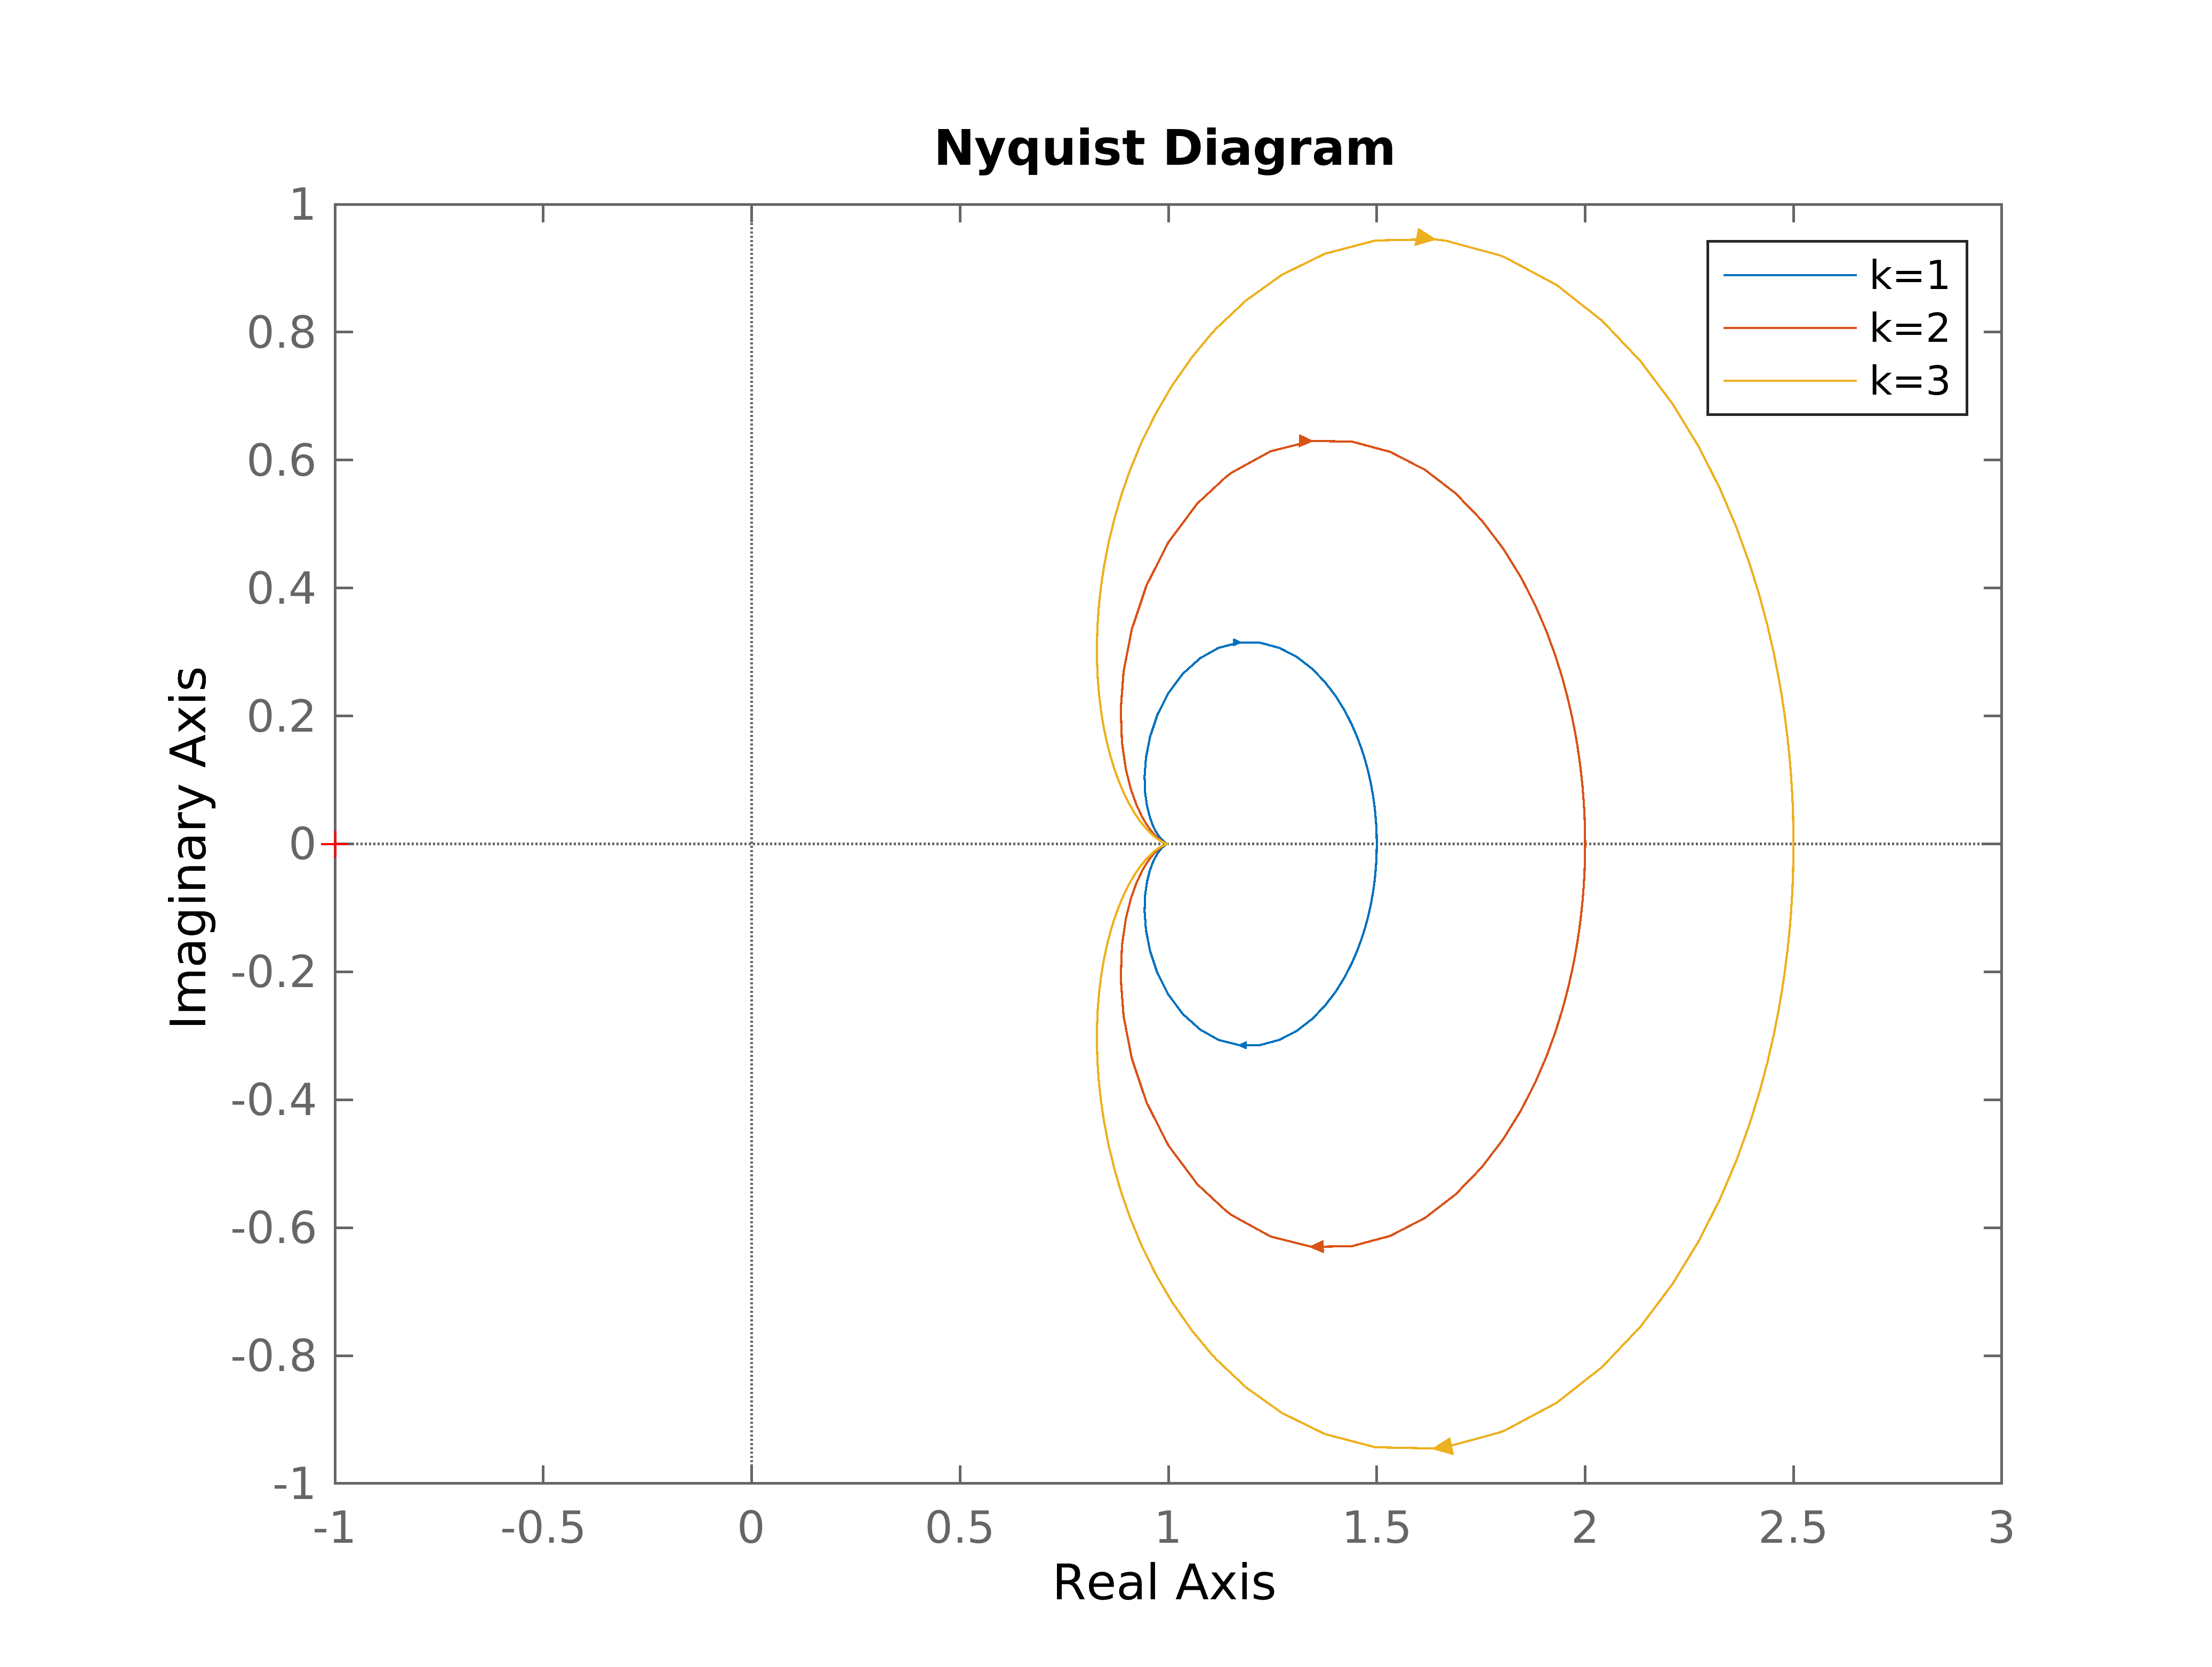
\includegraphics[scale=0.8]{a.png}
        \centering
    \end{figure}
    Rzeczywiscie widać, że, dla $k$ mniejszych od -2 system jest niestabilny.
    \newpage            

    \item[b)] $K=k, \ G=\frac{1}{\left(s + 1\right) \left(s + 2\right)}$
    Transmitancja CLS:
    $$K_Z=\frac{k}{1+KG}=\frac{k}{1+k\frac{1}{\left(s + 1\right) \left(s + 2\right)}}=\frac{k \left(s + 1\right) \left(s + 2\right)}{k + \left(s + 1\right) \left(s + 2\right)}$$
    Transmitancja OLS:
    $$K_O=K\cdot G=\frac{k}{\left(s + 1\right) \left(s + 2\right)}$$
    \textbf{Sprawdzamy stabilność CLS z pomocą kryterium Hurwitza:}\newline
    Wielomian charakterystyczny CLS:
    $$M_Z=k + \left(s + 1\right) \left(s + 2\right)$$
    Macierz Hurwitza na podstawie tego wielomianu oraz wartości wyznacznika i podwyznaczników:
    $$\left[\begin{matrix}3 & 0\\1 & k + 2\end{matrix}\right]$$
    $$\left[ 3 k + 6, \  3\right]$$
    Na podstawie kryterium Hurtwiza możemy stwierdzić, że CLS jest stabilne dla k<-2
    \newline\textbf{Sprawdzam stabilność CLS z pomocą kryterium Nyquista}\newline
    Używam kryterium hurtwiza do sprawdzenia kiedy OLS jest stabilny. OLS jest stabilny, dla dowolego k
    Wykres Nyquista dla 1+KG:
    %oceniam stabilnosc recznie
    \begin{figure}
        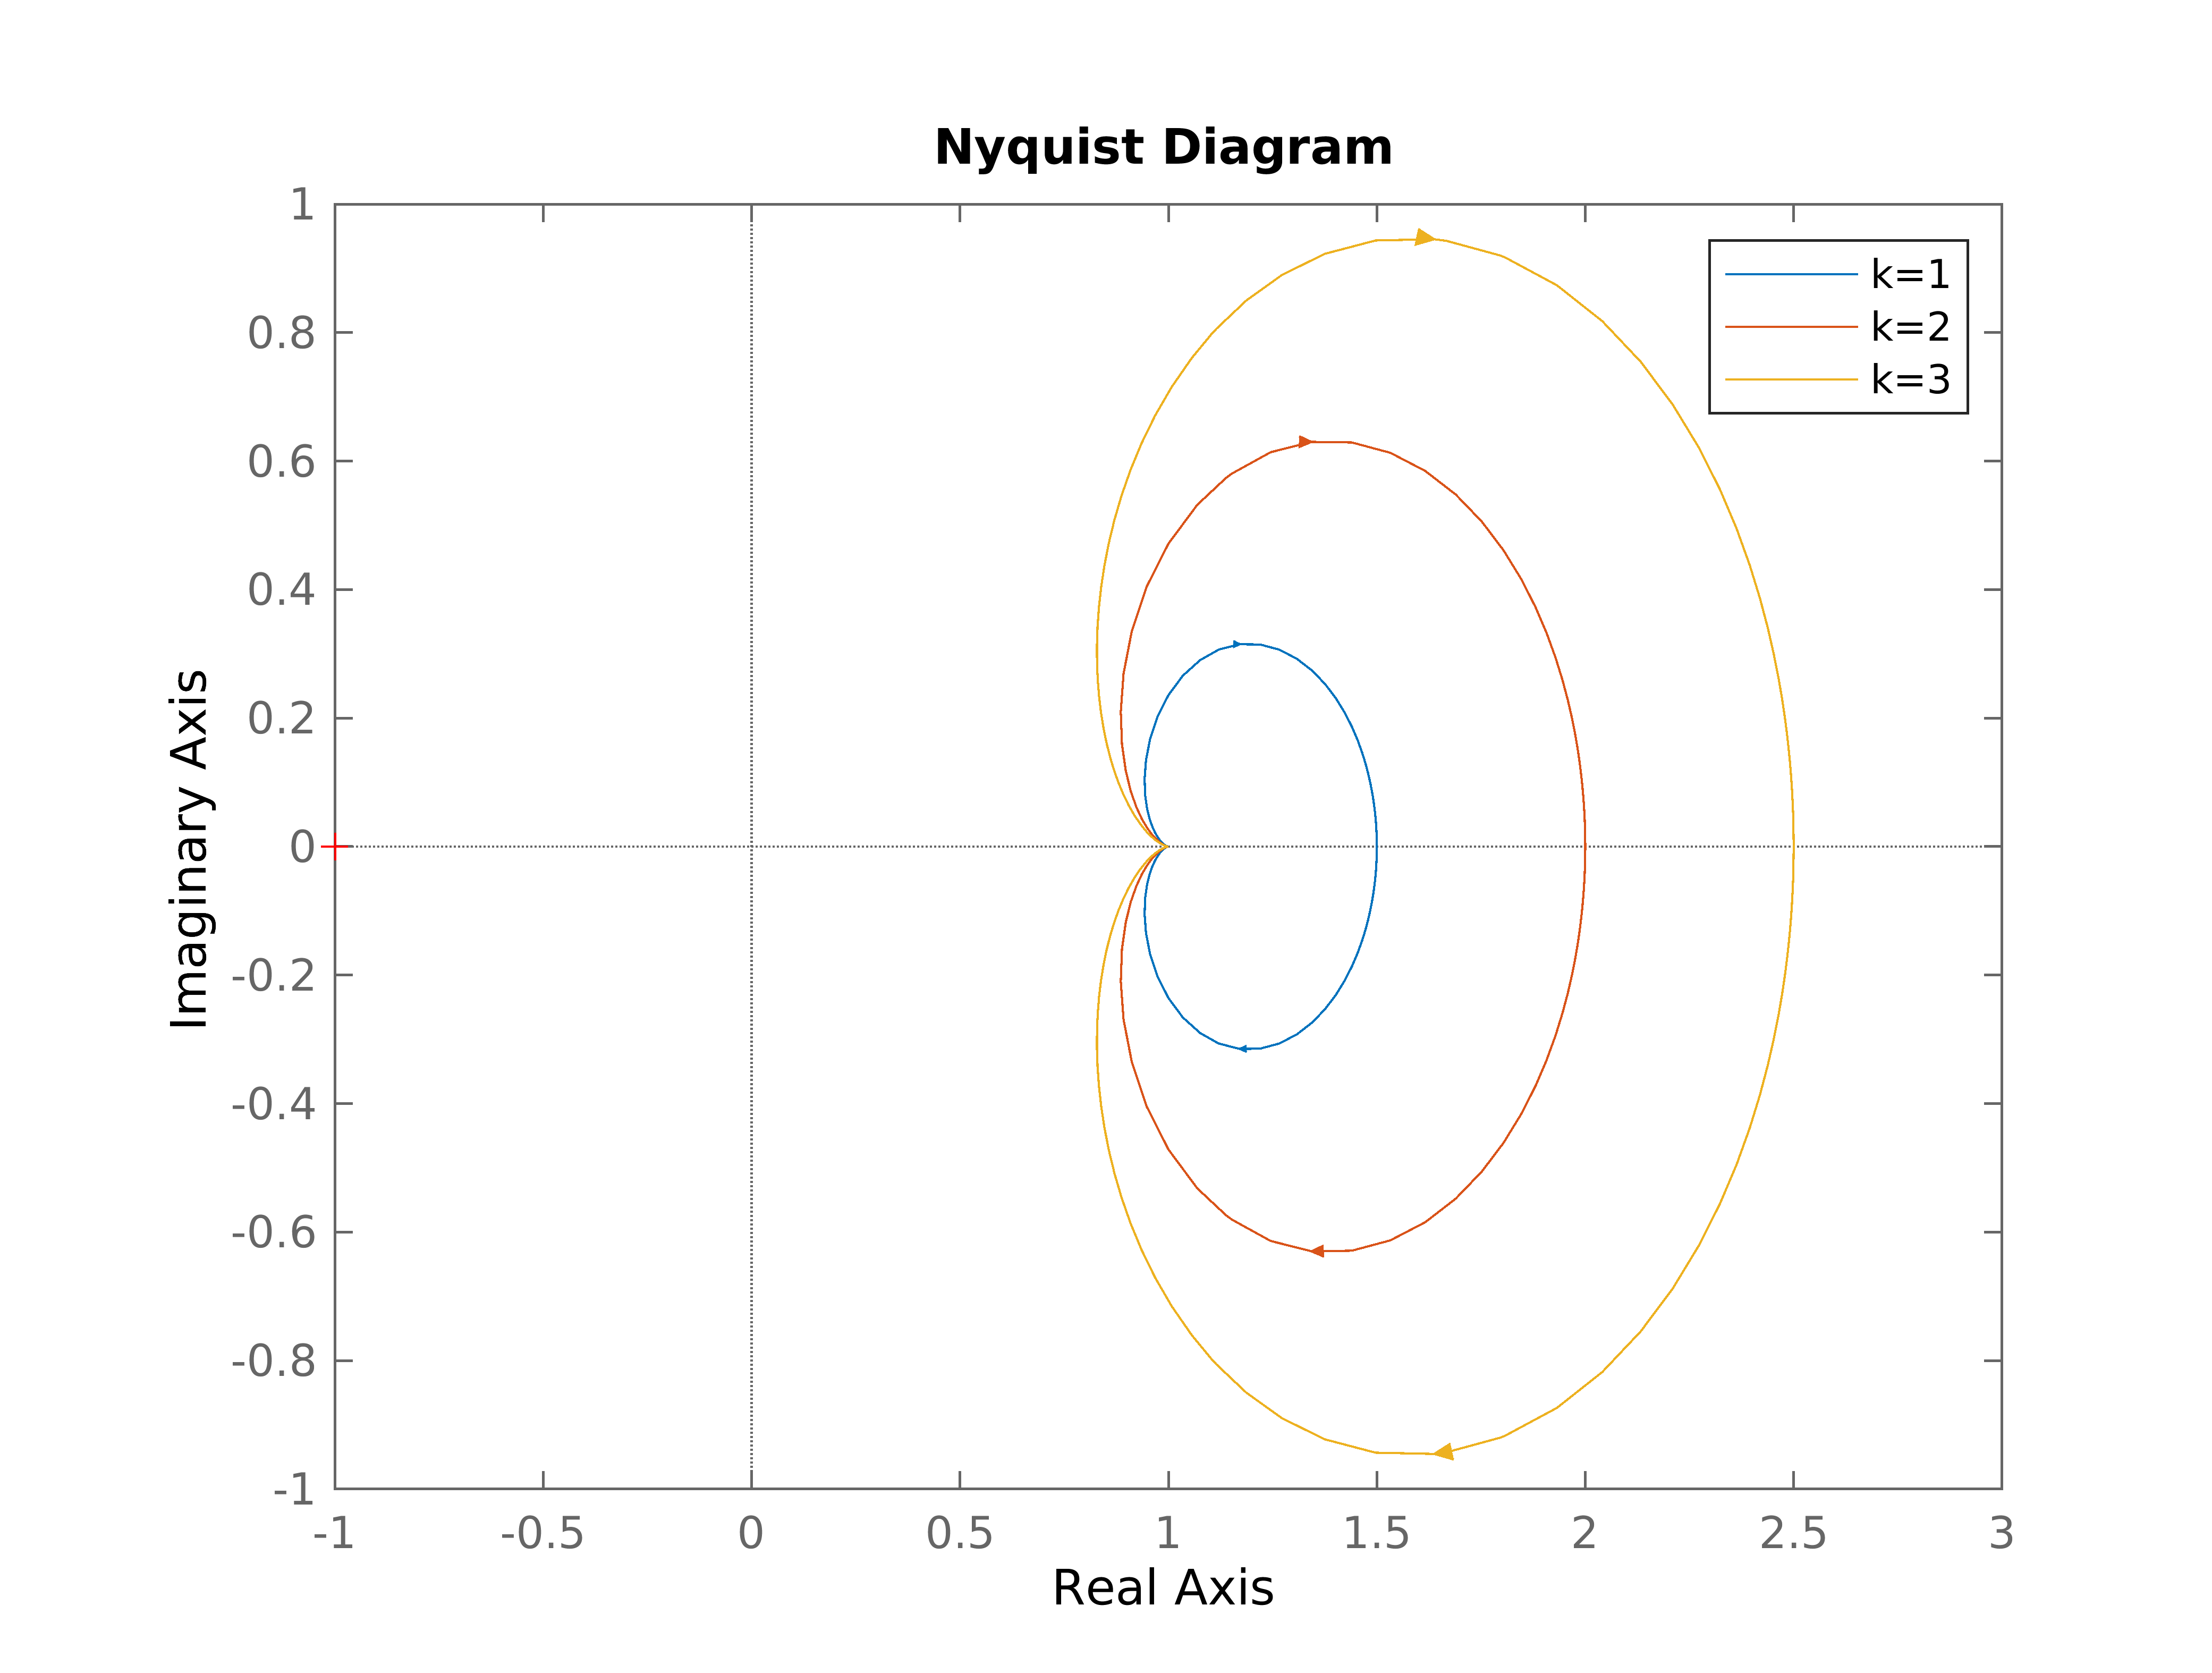
\includegraphics[scale=0.8]{b.png}
        \centering
    \end{figure}
    Na podsawie wykresu Nyuqista stwierdzam, że CLS jest stabilny dla k>-2
    \newpage
    
    \item[c)] $K=\frac{1}{s + 1}, G=\frac{1}{s + 3}$
    Transmitancja CLS:
    $$K_Z=\frac{k}{1+KG}=\frac{\frac{1}{s + 1}}{1+\frac{1}{s + 1}\frac{1}{s + 3}}=\frac{s + 3}{\left(s + 1\right) \left(s + 3\right) + 1}$$
    Transmitancja OLS:
    $$K_O=K\cdot G=\frac{1}{\left(s + 1\right) \left(s + 3\right)}$$
    \textbf{Sprawdzamy stabilność CLS z pomocą kryterium Hurwitza:}\newline
    Wielomian charakterystyczny CLS:
    $$M_Z=\left(s + 1\right) \left(s + 3\right) + 1$$
    Macierz Hurwitza na podstawie tego wielomianu oraz wartości wyznacznika i podwyznaczników:
    $$\left[\begin{matrix}4 & 0\\1 & 4\end{matrix}\right]$$
    $$\left[ 16, \  4\right]$$
    Według KH system jest stabilny.
    %oceniam stabilnosc recznie
    \newline\textbf{Sprawdzam stabilność CLS z pomocą kryterium Nyquista}\newline
    Używam kryterium hurtwiza do sprawdzenia czy OLS jest stabilny. OLS jest stabilny.
    Wykres Nyquista dla 1+KG:   
    %oceniam stabilnosc recznie
    \begin{figure}
        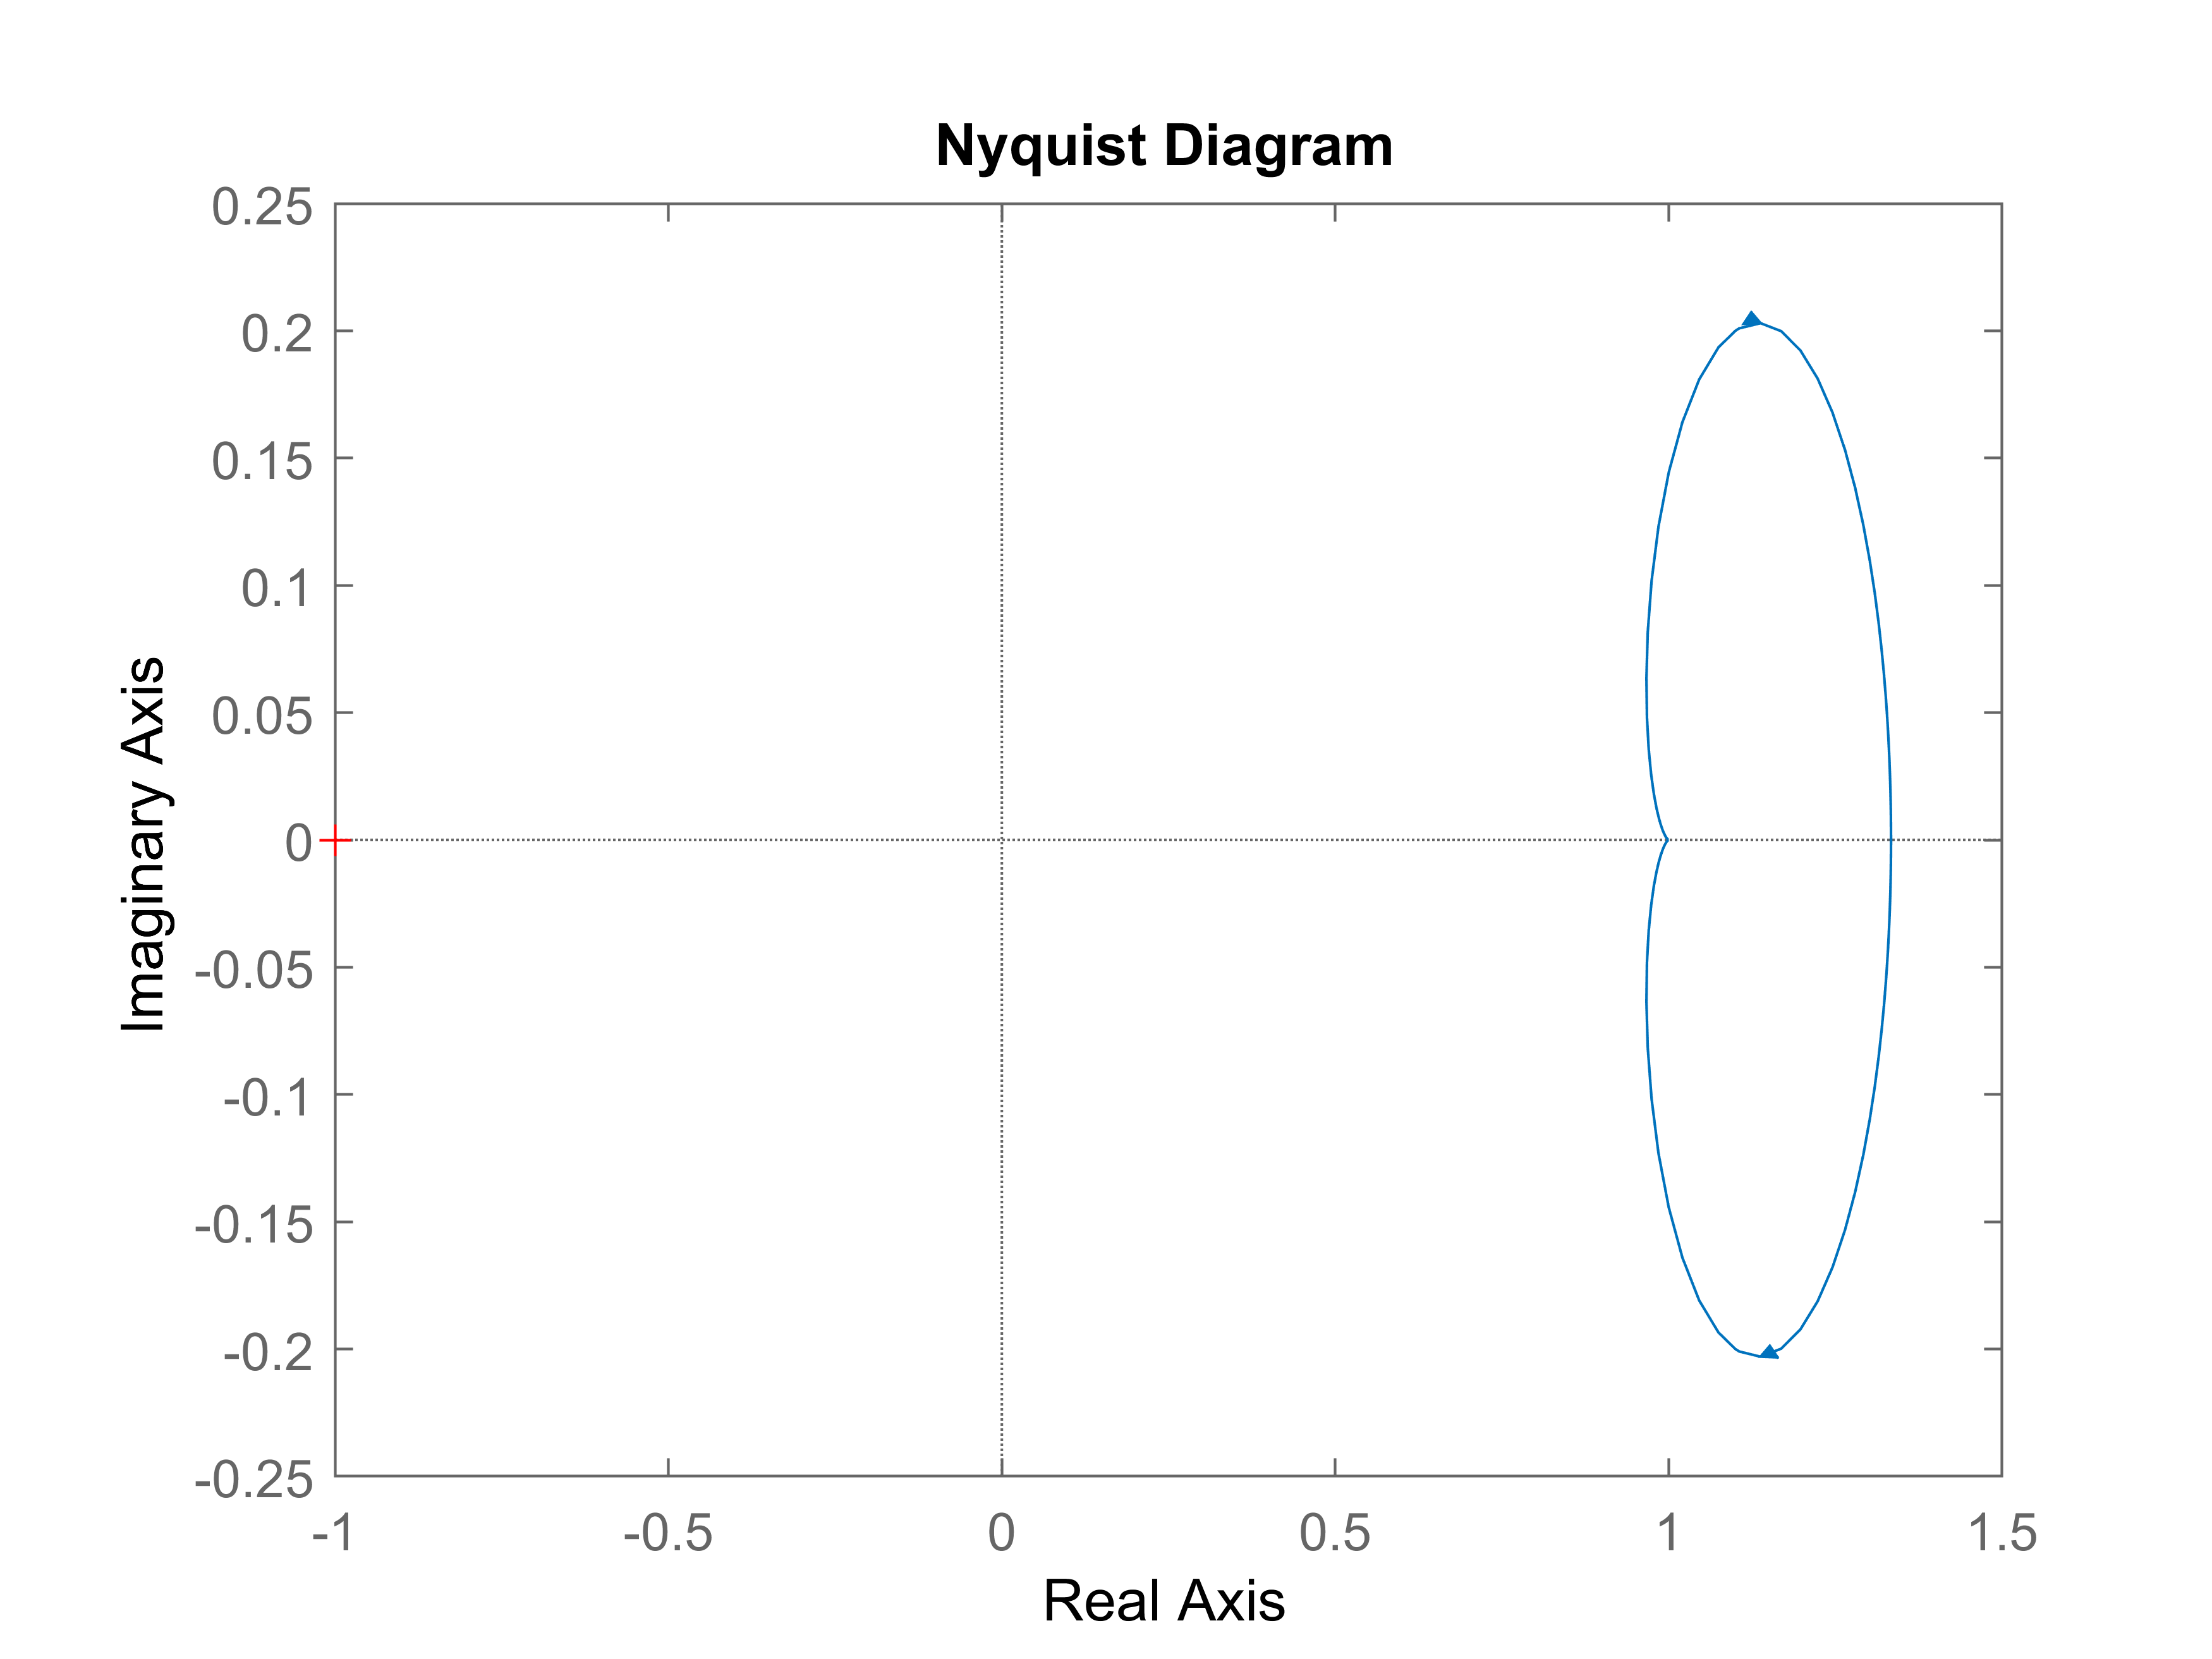
\includegraphics[scale=0.8]{c.png}
        \centering
    \end{figure}
    Na podsawie wykresu Nyuqista stwierdzam, że CLS jest stabilny
    \newpage            
        
    \item[d)] $K=\frac{1}{s^{2} + 4 s + 5}, G=\frac{1}{s + 3}$
    Transmitancja CLS:
    $$K_Z=\frac{k}{1+KG}=\frac{\frac{1}{s^{2} + 4 s + 5}}{1+\frac{1}{s^{2} + 4 s + 5}\frac{1}{s + 3}}=\frac{s + 3}{\left(s + 3\right) \left(s^{2} + 4 s + 5\right) + 1}$$
    Transmitancja OLS:
    $$K_O=K\cdot G=\frac{1}{\left(s + 3\right) \left(s^{2} + 4 s + 5\right)}$$
    \textbf{Sprawdzamy stabilność CLS z pomocą kryterium Hurwitza:}\newline
    Wielomian charakterystyczny CLS:
    $$M_Z=\left(s + 3\right) \left(s^{2} + 4 s + 5\right) + 1$$
    Macierz Hurwitza na podstawie tego wielomianu oraz wartości wyznacznika i podwyznaczników:
    $$\left[\begin{matrix}7 & 16 & 0\\1 & 17 & 0\\0 & 7 & 16\end{matrix}\right]$$
    $$\left[ 1648, \  103, \  7\right]$$
    Według KH system jest stabilny.
    %oceniam stabilnosc recznie
    \newline\textbf{Sprawdzam stabilność CLS z pomocą kryterium Nyquista}\newline
    Używam kryterium hurtwiza do sprawdzenia czy OLS jest stabilny. OLS jest stabilny.
    Wykres Nyquista dla 1+KG:
    %oceniam stabilnosc recznie
    \begin{figure}
        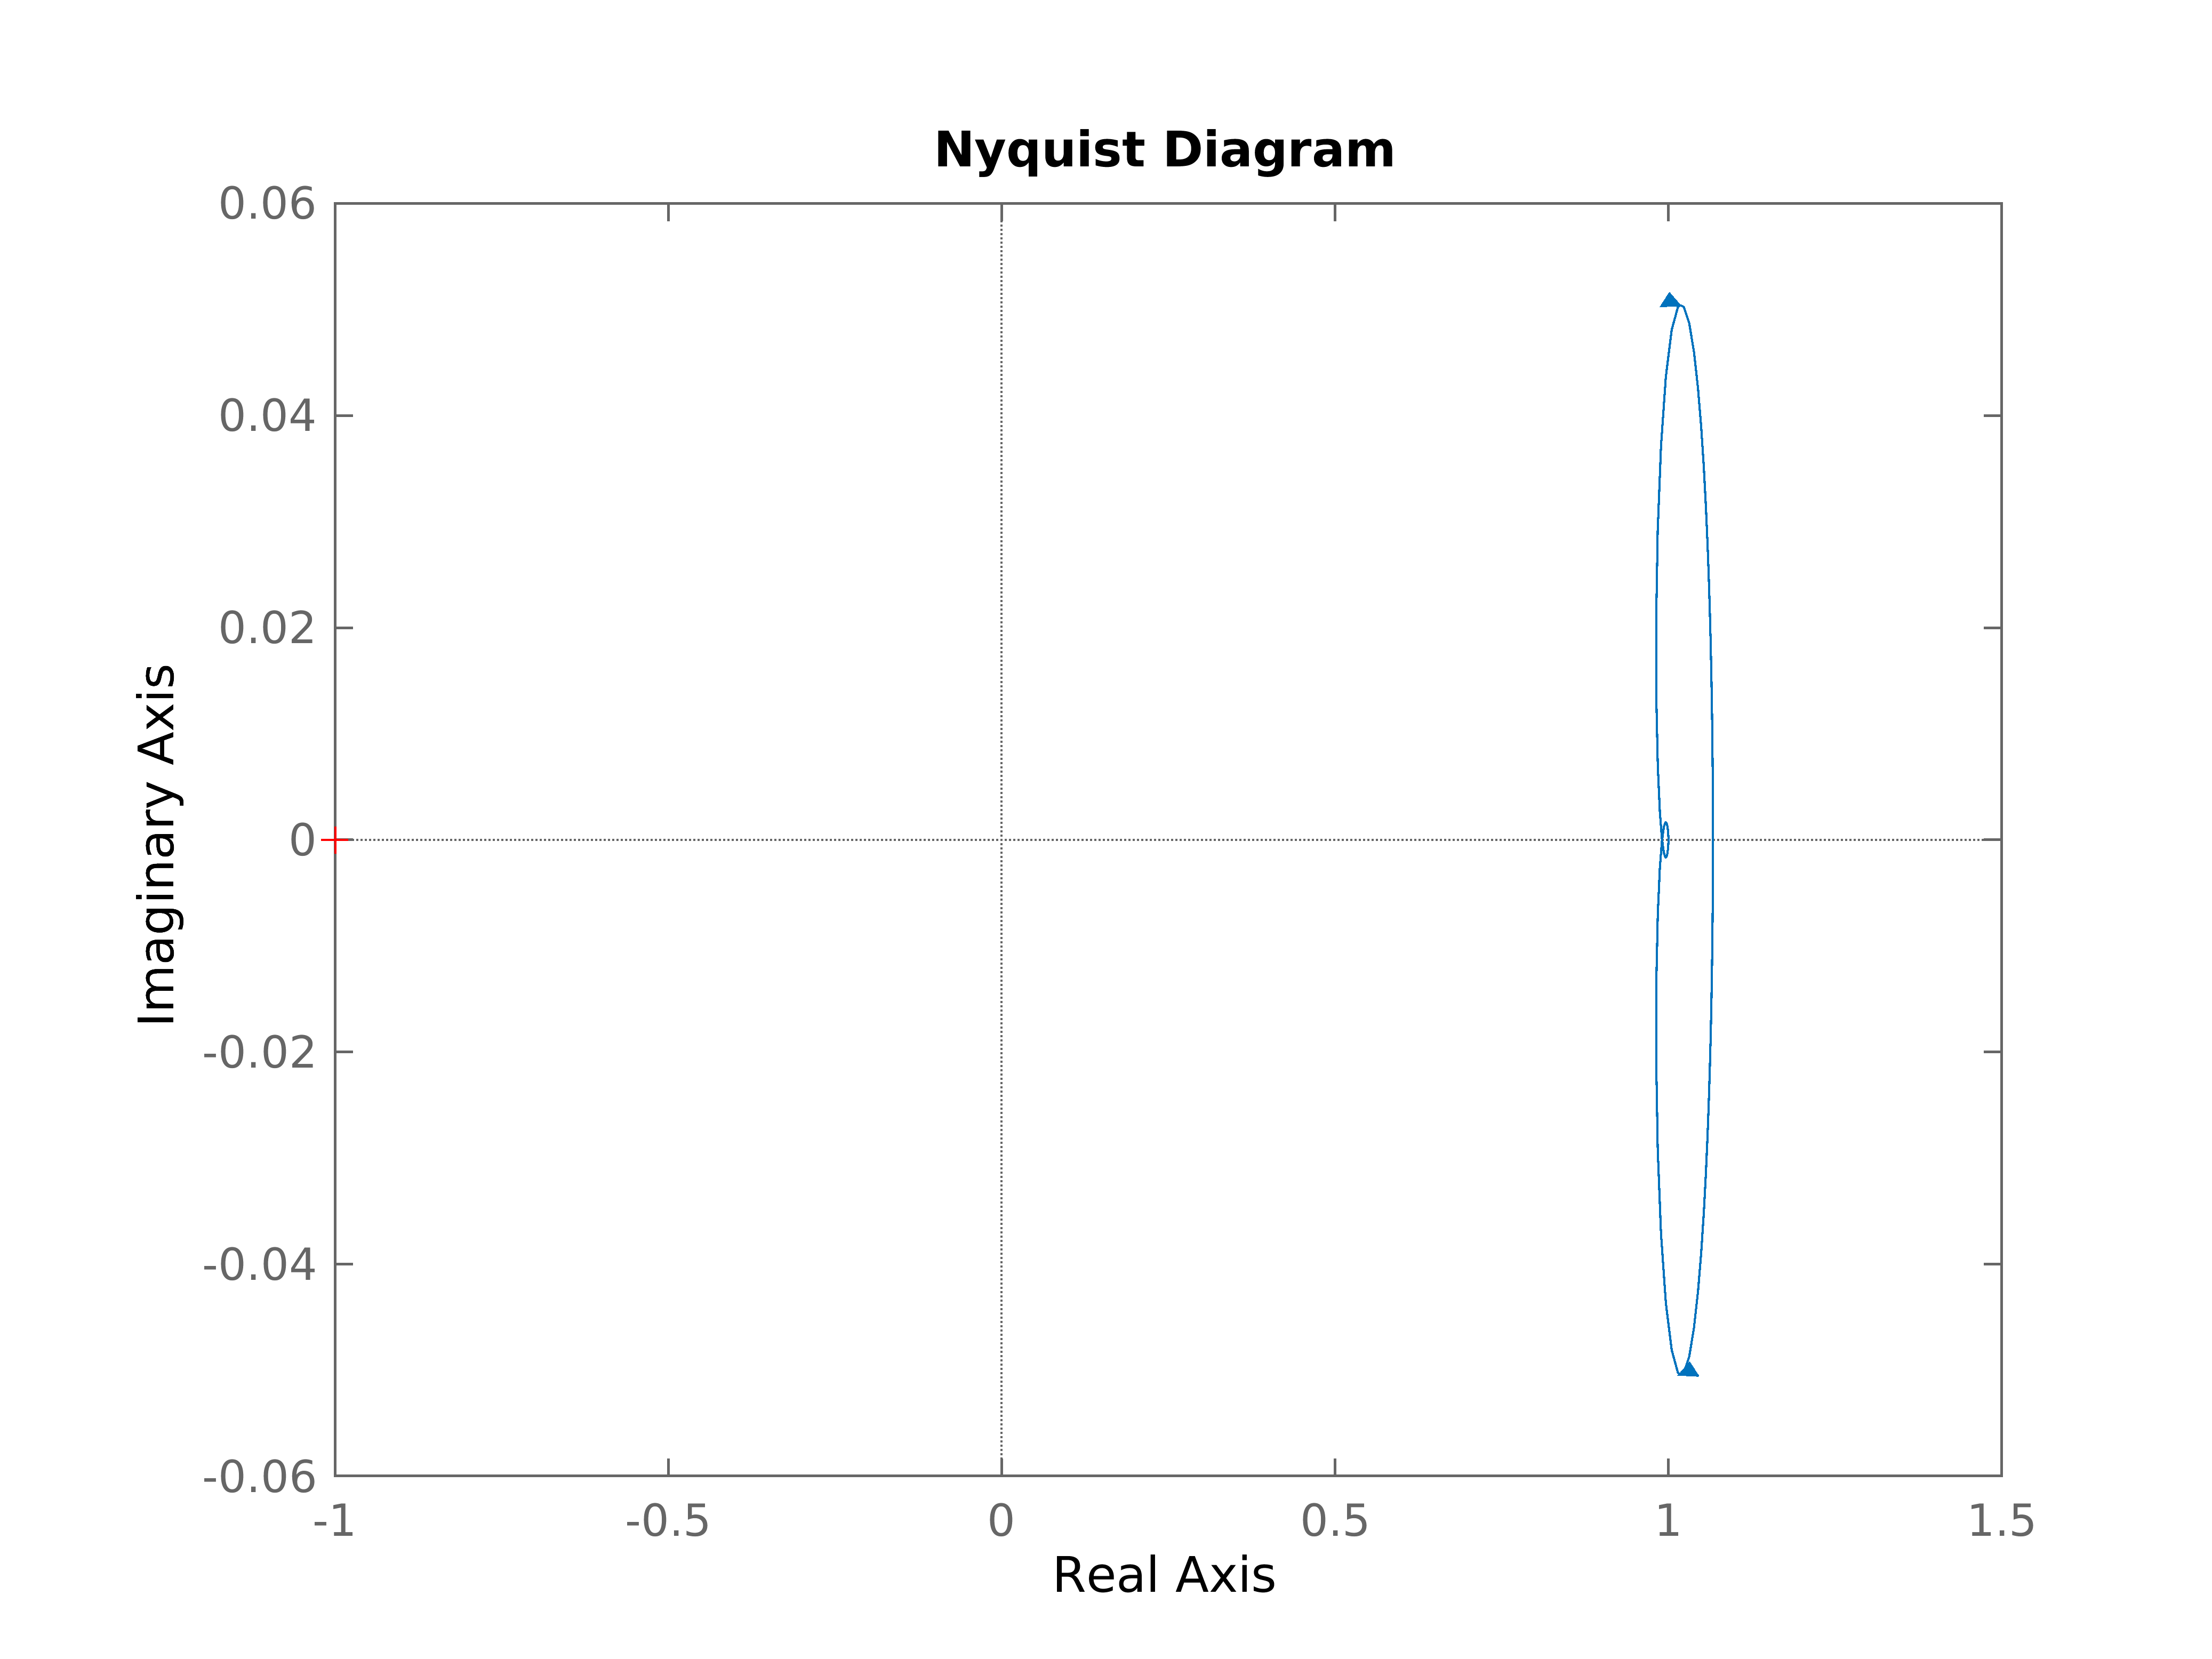
\includegraphics[scale=0.8]{d.png}
    \end{figure}
    Na podsawie wykresu Nyuqista stwierdzam, że CLS jest stabilny
    \newpage            

\end{itemize}
\end{document}
